\taskpic{ Для облегчения подъёма грузов часто применяют ворот,
  состоящий из двух валов, неподвижно закреплённых на одной оси. При
  работе такого ворота трос, сматываясь с одного вала, одновременно
  наматывается на другой. Какую силу $F$ нужно приложить к рукоятке
  ворота длиной $l$, чтобы груз массы $m$ находился в равновесии?
  Весом блока и трением пренебречь. Радиус малого вала $r$, большого
  --- $R$. }  {
  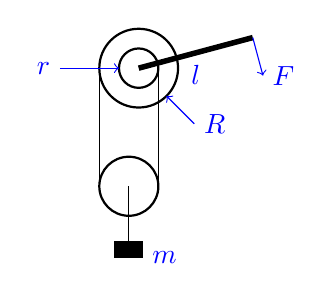
\begin{tikzpicture}
    \draw[thick] (2,3.5) circle (0.25);
    \draw[thick] (2,3.5) circle (0.5);
    \draw (2.25,3.5) -- (2.25,2);
    \draw (1.5,3.5) -- (1.5,2);
    \draw[thick] (1.875,2) circle (0.375);
    \draw (1.875,2) -- (1.875,1.3);
    \draw[fill=black] (1.7,1.3) rectangle (2.05,1.1) node[right,blue]
    {$m$};
    \draw[line width=0.07cm] (2,3.5) -- ++(15:1.5cm)
    node[midway,below,blue] {$l$};
    \draw[blue,->] (2,3.5) ++ (15:1.5cm) -- ++(-75:0.5cm)
    node[right,blue] {$F$};
    \draw[blue,->] (2,3.5) ++(-45:1cm) node[right] {$R$} --
    ++(135:0.5cm);
    \draw[blue,->] (1,3.5) node[left] {$r$} -- (1.75,3.5);
  \end{tikzpicture}
}
% Лукашик, 14.24